%%%%%%%%%%%%%%%%%%%%%%%%%%%%%%%%%%%%%%%%%%%%%%%%%%%%%%%%
%%
\clearpage
\newpage
\section{The cal\_FF recipe}
\label{ch:the_recipes:cal_FF_RAW_spirou}
%%
%%%%%%%%%%%%%%%%%%%%%%%%%%%%%%%%%%%%%%%%%%%%%%%%%%%%%%%%

Creates the flat fields. \\ 

% -------------------------------------------------------
\subsection{The inputs}
% -------------------------------------------------------
The input of \calFFraw is as follows:
\begin{cmdbox}
cal_FF_RAW_spirou.py night_repository filenames
\end{cmdbox}
\noindent for example
\begin{cmdbox}[title={example}]
cal_FF_RAW_spirou.py 20170710 dark_flat02f10.fits dark_flat03f10.fits dark_flat04f10.fits dark_flat05f10.fits dark_flat06f10.fits
\end{cmdbox}
\noindent or
\begin{pythonbox}
import cal_FF_RAW_spirou
night_repository = '20170710'
filenames = ['dark_flat02f10.fits', 'dark_flat03f10.fits', 'dark_flat04f10.fits', 
             'dark_flat05f10.fits', 'dark_flat06f10.fits']
cal_FF_RAW_spirou.main()
\end{pythonbox}

\noindent where `night\_repository' defines \argnightname and `filenames' define the list of files in \argfilenames. All files in filenames must be valid python strings separated by a space (command line) or in a line (python) and must have the following prefixes:
\begin{itemize}
	\item dark\_flat
	\item flat\_dark
\end{itemize}

% -------------------------------------------------------
\subsection{The outputs}
% -------------------------------------------------------
The outputs of \calFFraw are as follows:

\begin{itemize}

\item \definevariable{text:blazefits}{blazefits} in form:
\begin{tcustomdir}
\{\reduceddir\}/\{date prefix\}\_\{file\}\_blaze\_\{fiber\}.fits
\end{tcustomdir}

\item \definevariable{text:flatfits}{flatfits} in form:
\begin{tcustomdir}
\{\reduceddir\}/\{date prefix\}\_\{file\}\_flat\_\{fiber\}.fits
\end{tcustomdir}

\end{itemize}


\noindent where `date prefix' is constructed from \argnightname and the file name is the first file in \argfilenames.


\noindent for example for \reduceddir\lstinline[style=pythoninline]|='/drs/data/reduced/20170710'| and \argfilenames\lstinline[style=pythoninline]|=['dark_flat02f10.fits', 'dark_flat03f10.fits', 'dark_flat04f10.fits', 'dark_flat05f10.fits', 'dark_flat06f10.fits']| the output files would be:
\begin{tcustomdir}
\begin{itemize}
\item \path{/drs/data/reduced/20170710/20170710_flat_dark02f10_blaze_AB.fits}
\item \path{/drs/data/reduced/20170710/20170710_flat_dark02f10_flat_AB.fits}
\end{itemize}
\end{tcustomdir}

% -------------------------------------------------------
\subsection{Summary of procedure}
% -------------------------------------------------------
\begin{enumerate}
\item adds all `dark\_flat' or `flat\_dark' files together
\item corrects for darks
\item resizes the image
\item possible background subtraction?
\item extracts the orders using tilt and weight
\item calculates the blaze
\item calculates the flat field, (flat = extraction / blaze)
\item stores the flat fields
\item does some quality control
\item updates calibDB with key "FLAT\_\{fiber\}" where \{fiber\} = [AB, C] etc.
\end{enumerate}

% -------------------------------------------------------
\subsection{Quality Control}
% -------------------------------------------------------

There is currently one quality control check for \calFFraw
\begin{itemize}
\item Too much flux in the image: 
\begin{thighlight}
\begin{equation}
\text{maximum signal} > \text{\definevariable{text:qc_max_signal}{qc\_max\_signal}} * \text{\definevariable{text:nbframes}{nbframes}}
\end{equation}
\end{thighlight}
\end{itemize}
\begin{note}
This check does not currently lead to a failed run and all files are processed as passing quality checks
\end{note}

\noindent The output file is passed into the \calibdb with key `FLAT\_\{fiber\}' for the `\definevariable{text:flatfits}{flatfits}' file. \\

\noindent For example the following lines are added to the \calibdb for 
\argnightname{\lstinline[style=pythoninline]| = "20170710" |} and \argfilenames{\lstinline[style=pythoninline]|=['dark_flat02f10.fits', 'dark_flat03f10.fits', 'dark_flat04f10.fits', 'dark_flat05f10.fits', 'dark_flat06f10.fits']|}. \\

\begin{textbox}[title={In calibration database file}]
FLAT_C 20170710 20170710_dark_flat02f10_flat_C.fits 2017-07-10-13:03:50.440000 1499691830.44
BLAZE_C 20170710 20170710_dark_flat02f10_blaze_C.fits 2017-07-10-13:03:50.440000 1499691830.44
\end{textbox}


% -------------------------------------------------------
\newpage
\subsection{Example working run}
% -------------------------------------------------------

An example run where everything worked is below:
\begin{cmdbox}[title={example}]
cal_FF_RAW_spirou.py 20170710 dark_flat02f10.fits dark_flat03f10.fits dark_flat04f10.fits dark_flat05f10.fits dark_flat06f10.fits
\end{cmdbox}
\begin{cmdboxprintspecial}[fontupper=\tiny, fontlower=\tiny]
@gHH:MM:SS.S -   || *****************************************@g
@gHH:MM:SS.S -   || * SPIROU \@(#) Geneva Observatory (VERSION)@g
@gHH:MM:SS.S -   || *****************************************@g
@gHH:MM:SS.S -   ||(dir_data_raw)      DRS_DATA_RAW=/drs/data/raw@g
@gHH:MM:SS.S -   ||(dir_data_reduc)    DRS_DATA_REDUC=/drs/data/reduced@g
@gHH:MM:SS.S -   ||(dir_calib_db)      DRS_CALIB_DB=/drs/data/calibDB@g
@gHH:MM:SS.S -   ||(dir_data_msg)      DRS_DATA_MSG=/drs/data/msg@g
@gHH:MM:SS.S -   ||(print_level)       PRINT_LEVEL=all         %(error/warning/info/all)@g
@gHH:MM:SS.S -   ||(log_level)         LOG_LEVEL=all         %(error/warning/info/all)@g
@gHH:MM:SS.S -   ||(plot_graph)        DRS_PLOT=1            %(def/undef/trigger)@g
@gHH:MM:SS.S -   ||(used_date)         DRS_USED_DATE=undefined@g
@gHH:MM:SS.S -   ||(working_dir)       DRS_DATA_WORKING=/drs/data/tmp@g
@gHH:MM:SS.S -   ||                    DRS_INTERACTIVE is not set, running on-line mode@g
@gHH:MM:SS.S -   ||                    DRS_DEBUG is set, debug mode level:1@g
@gHH:MM:SS.S -   |cal_FF_RAW_spirou:02f10+[...]|Now running : cal_FF_RAW_spirou on file(s): dark_flat02f10.fits, dark_flat03f10.fits, dark_flat04f10.fits, dark_flat05f10.fits, dark_flat06f10.fits@g
@gHH:MM:SS.S -   |cal_FF_RAW_spirou:02f10+[...]|On directory /drs/data/raw/20170710@g
@gHH:MM:SS.S -   |cal_FF_RAW_spirou:02f10+[...]|ICDP_NAME loaded from: /scratch/Projects/spirou_py3/spirou_py3/INTROOT/config/constants_SPIROU.py@g
@gHH:MM:SS.S - * |cal_FF_RAW_spirou:02f10+[...]|Correct type of image for Flat-field (dark_flat or flat_dark)@g
@gHH:MM:SS.S -   |cal_FF_RAW_spirou:02f10+[...]|Calibration file: 20170710_flat_flat02f10_badpixel.fits already exists - not copied@g
@gHH:MM:SS.S -   |cal_FF_RAW_spirou:02f10+[...]|Calibration file: 20170710_dark_dark02d406.fits already exists - not copied@g
...
@gHH:MM:SS.S -   |cal_FF_RAW_spirou:02f10+[...]|Calibration file: 20170710_flat_dark02f10_order_profile_AB.fits already exists - not copied@g
@gHH:MM:SS.S -   |cal_FF_RAW_spirou:02f10+[...]|Calibration file: 20170710_dark_flat02f10_order_profile_C.fits already exists - not copied@g
@gHH:MM:SS.S -   |cal_FF_RAW_spirou:02f10+[...]|Calibration file: 20170710_fp_fp02a203_tilt.fits already exists - not copied@g
@gHH:MM:SS.S -   |cal_FF_RAW_spirou:02f10+[...]|Calibration file: spirou_wave_ini3.fits already exists - not copied@g
@gHH:MM:SS.S -   |cal_FF_RAW_spirou:02f10+[...]|Calibration file: 2017-10-11_21-32-17_hcone_hcone02c406_wave_AB.fits already exists - not copied@g
@gHH:MM:SS.S -   |cal_FF_RAW_spirou:02f10+[...]|Calibration file: spirou_wave_ini3.fits already exists - not copied@g
@gHH:MM:SS.S -   |cal_FF_RAW_spirou:02f10+[...]|Calibration file: 2017-10-11_21-32-17_hcone_hcone02c406_wave_C.fits already exists - not copied@g
@gHH:MM:SS.S - * |cal_FF_RAW_spirou:02f10+[...]|Now processing Image TYPE UNKNOWN with cal_FF_RAW_spirou recipe@g
@gHH:MM:SS.S -   |cal_FF_RAW_spirou:02f10+[...]|Reading Image /drs/data/raw/20170710/dark_flat02f10.fits@g
@gHH:MM:SS.S -   |cal_FF_RAW_spirou:02f10+[...]|Image 2048 x 2048 loaded@g
@gHH:MM:SS.S - * |cal_FF_RAW_spirou:02f10+[...]|Adding 4 frame(s)@g
@gHH:MM:SS.S -   |cal_FF_RAW_spirou:02f10+[...]|Reading File: /drs/data/raw/20170710/dark_flat03f10.fits@g
@gHH:MM:SS.S -   |cal_FF_RAW_spirou:02f10+[...]|Reading File: /drs/data/raw/20170710/dark_flat04f10.fits@g
@gHH:MM:SS.S -   |cal_FF_RAW_spirou:02f10+[...]|Reading File: /drs/data/raw/20170710/dark_flat05f10.fits@g
@gHH:MM:SS.S -   |cal_FF_RAW_spirou:02f10+[...]|Reading File: /drs/data/raw/20170710/dark_flat06f10.fits@g
@gHH:MM:SS.S -   |cal_FF_RAW_spirou:02f10+[...]|Doing Dark Correction using /drs/data/calibDB/20170710_dark_dark02d406.fits@g
@gHH:MM:SS.S -   |cal_FF_RAW_spirou:02f10+[...]|Image format changed to 2035x1930@g
@gHH:MM:SS.S - * |cal_FF_RAW_spirou:02f10+[...]|Nb dead pixels = 568541 / 14.48 %@g
@gHH:MM:SS.S - * |cal_FF_RAW_spirou:02f10+[...]|Maximum average flux/pixel in the spectrum: 73636.3 [ADU]@g
@gHH:MM:SS.S -   |cal_FF_RAW_spirou:02f10+[...]|Reading localization parameters of Fiber C@g
@gHH:MM:SS.S -   |cal_FF_RAW_spirou:02f10+[...]C|Reading order profile of Fiber C@g
@gHH:MM:SS.S -   |cal_FF_RAW_spirou:02f10+[...]|On fiber C order 0: S/N= 1158.4  - FF rms=4.68 %@g
@gHH:MM:SS.S -   |cal_FF_RAW_spirou:02f10+[...]|On fiber C order 1: S/N= 1193.9  - FF rms=4.80 %@g
@gHH:MM:SS.S -   |cal_FF_RAW_spirou:02f10+[...]|On fiber C order 2: S/N= 1232.6  - FF rms=4.76 %@g
...
@gHH:MM:SS.S -   |cal_FF_RAW_spirou:02f10+[...]|On fiber C order 33: S/N= 1686.9  - FF rms=5.67 %@g
@gHH:MM:SS.S -   |cal_FF_RAW_spirou:02f10+[...]|On fiber C order 34: S/N= 1574.5  - FF rms=8.17 %@g
@gHH:MM:SS.S -   |cal_FF_RAW_spirou:02f10+[...]|On fiber C order 35: S/N= 1260.6  - FF rms=8.10 %@g
@gHH:MM:SS.S -   |cal_FF_RAW_spirou:02f10+[...]C|Saving blaze spectrum for fiber: C in 20170710_dark_flat02f10_blaze_C.fits@g
@yHH:MM:SS.S - \@ |python warning Line 980  warning reads: Card is too long, comment will be truncated.|@y
@gHH:MM:SS.S -   |cal_FF_RAW_spirou:02f10+[...]C|Saving FF spectrum for fiber: C in 20170710_dark_flat02f10_flat_C.fits@g
@yHH:MM:SS.S - \@ |python warning Line 980  warning reads: Card is too long, comment will be truncated.|@y
@gHH:MM:SS.S - * |cal_FF_RAW_spirou:02f10+[...]|QUALITY CONTROL SUCCESSFUL - Well Done -@g
@gHH:MM:SS.S - * |cal_FF_RAW_spirou:02f10+[...]|Updating Calib Data Base with FLAT_C@g
@gHH:MM:SS.S - * |cal_FF_RAW_spirou:02f10+[...]|Updating Calib Data Base with BLAZE_C@g
@gHH:MM:SS.S - * |cal_FF_RAW_spirou:02f10+[...]|Recipe cal_FF_RAW_spirou has been successfully completed@g

\end{cmdboxprintspecial}


% -------------------------------------------------------
\newpage
\subsection{Interactive mode}
% -------------------------------------------------------

\noindent In interactive mode three figures will also appear (see Figure \ref{figure:cal_FF_raw_spirou}).

\begin{figure}

\begin{center}
\begin{minipage}{.495\textwidth}
\begin{center}
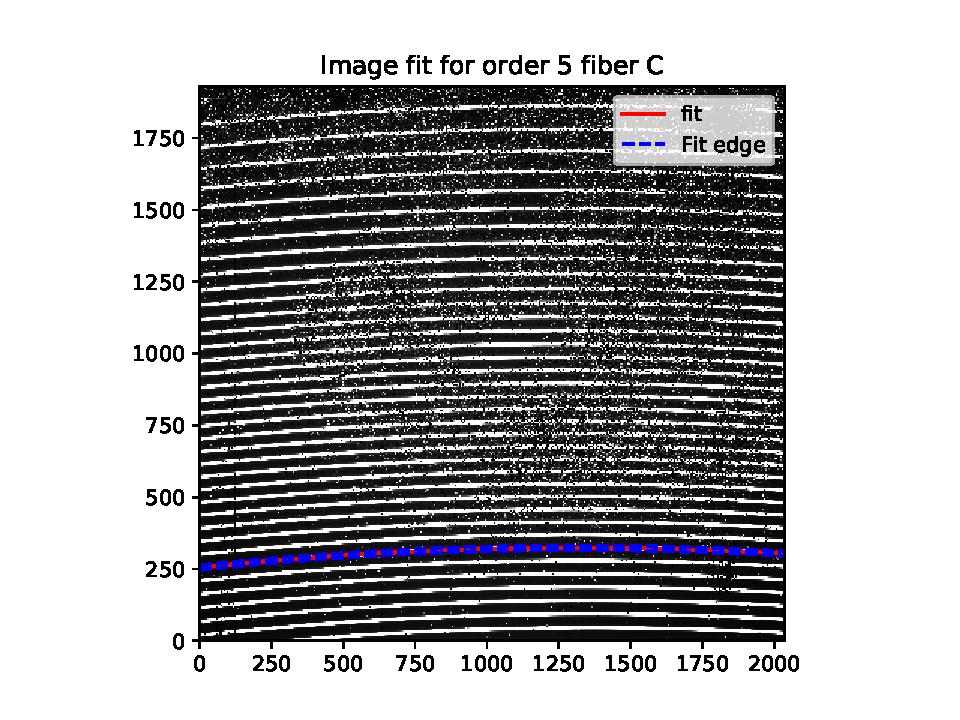
\includegraphics[width=\textwidth]{Figures/cal_FF_raw_spirou_1.pdf}
a
\end{center}
\end{minipage}%
\begin{minipage}{.495\textwidth}
\begin{center}
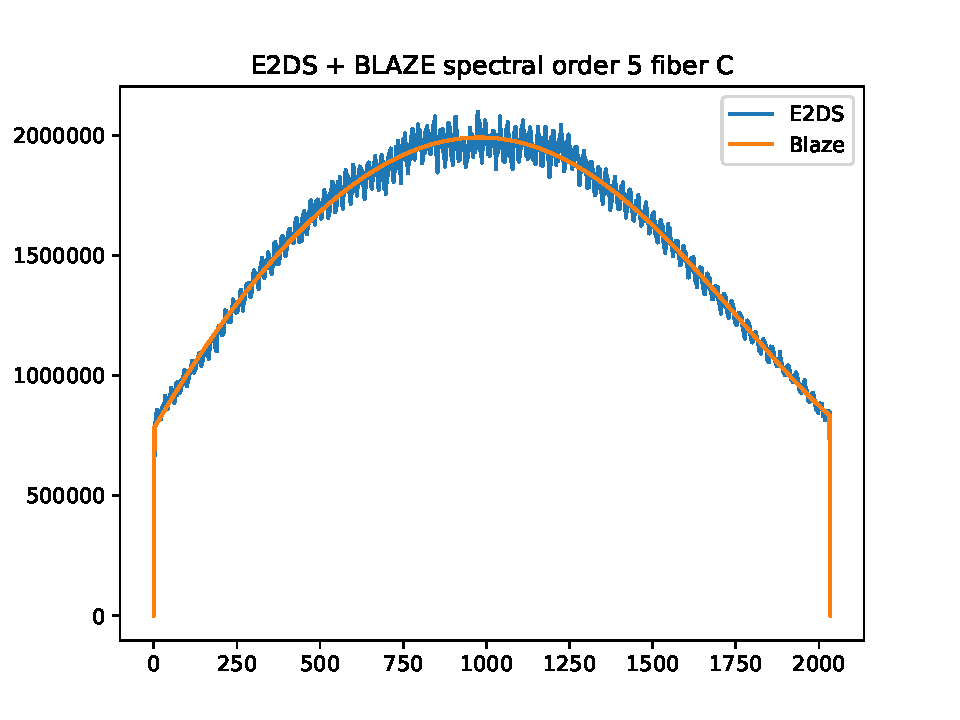
\includegraphics[width=\textwidth]{Figures/cal_FF_raw_spirou_2.pdf}
b
\end{center}
\end{minipage}%
\end{center}

\begin{center}
\begin{minipage}{.495\textwidth}
\begin{center}
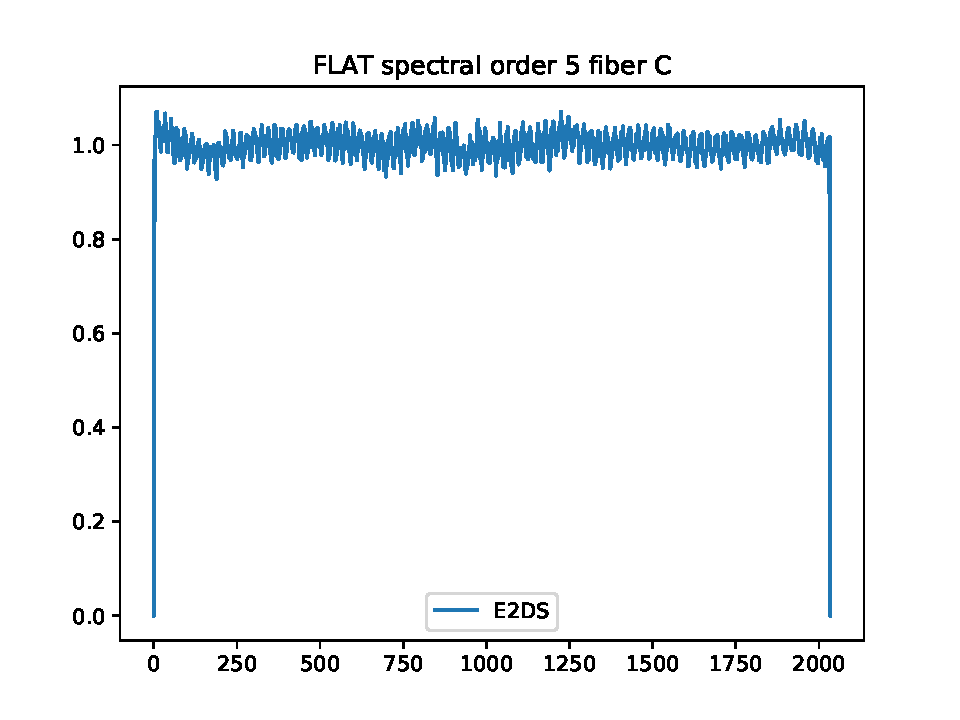
\includegraphics[width=\textwidth]{Figures/cal_FF_raw_spirou_3.pdf}
c
\end{center}
\end{minipage}%
\end{center}

\caption{\textbf{(a)} the full processed image with one order fit highlighted. \textbf{(b)} An extracted over-plotted with the blaze fit. \textbf{(c)}  A flattened order. \label{figure:cal_FF_raw_spirou}}
\end{figure}